\section{Coherent quantum state storage and transfer between two phase qubits via a resonant cavity \label{sec:coherentStateStorageBetweenPhaseQubits}}
 \iframe{Observed vacuum-Rabi splittings, vacuum-Rabi oscillations, and the
coherent transfer and storage of quantum states mediated by the
cavity.}
	A phase qubit, as described in Sec.~\ref{sec:autlerEffectThreeLevelSystem} is used. The states exist in phase space, and the lowest two are used. The flux can be controlled with:
	\begin{itemize}
		\item DC bias, giving a steady flux;
		\item 20GHz RF bias to jump in the flux
	\end{itemize}
		 	\ipic{2cm}{phij} \ipic{2cm}{coherentStateStorageBetweenPhaseQubits1}
		 	
	The eigenstates of the system are as in Ch.~\ref{sec:CavityQunatumElectrodynamics}:
	
	 \iframe{
		\[
		\begin{aligned}
		\iket{+,N} & = U^{\dagger}\ket{\tilde{1}} 				= \bigg(\cos(\theta/2)\mathbb{I}-i\sin(\theta/2)\sigma_y\bigg)
		\begin{pmatrix}1\\0 \end{pmatrix} = 
		\begin{pmatrix} \cos(\theta/2)\\\sin(\theta/2)\end{pmatrix} \\
		\iket{-,N} & = U^{\dagger}\ket{\tilde{0}} = \begin{pmatrix}
		-\sin(\theta/2)\\\cos(\theta/2)
		\end{pmatrix} \equiv -\sin(\theta/2)\iket{\uparrow,N} + \cos(\theta/2)\iket{\downarrow,N+1}\\
		\\
		 \mathcal{H}_{\text{middle}} 
		& = \kbordermatrix{&\ket{\uparrow,N} & \ket{\downarrow,N+1}\\
			\bra{\uparrow,N} & \blue{\hbar\omega_r(N+\frac{1}{2}) + \hbar\Delta} & \red{g_0\sqrt{N+1}}\\
			\bra{\downarrow,N+1} & \red{g_0\sqrt{N+1}} & \blue{\hbar\omega_r(N+\frac{1}{2}) - \hbar\Delta}}
		\quad \text{E}_{\pm} = \hbar\omega_r(N+\frac{1}{2}) \pm \frac{E_\text{coupled}}{2}
		\end{aligned}
	\]}
	  
	  For a single photon, $ N = 1 $, and on resonance, $ \Delta = 0 $ the entangled states are
	  
	  \[
	  \iket{\pm,1} = \frac{\iket{\uparrow,0} \pm \iket{\downarrow,1}}{\sqrt{2}} \quad E =  \hbar\omega_r/2 \pm g_0,\quad \mathcal{H}  = \kbordermatrix{&\ket{\uparrow,0} & \ket{\downarrow,1}\\
	  	\bra{\uparrow,0} & \blue{\hbar\omega_r/2} & \red{g_0}\\
	  	\bra{\downarrow,1} & \red{g_0} & \blue{\hbar\omega_r/2}}\\ 
	  \]
	  
	    \ipic{5cm}{cavityPic2}
	  
	  \noindent So putting the atom into \iket{\iup,0}, \textbf{not eigenstate} of the Hamiltonian $ \kbordermatrix{&\ket{\uparrow,0} & \ket{\downarrow,1}\\
	  	\bra{\uparrow,0} & \blue{\hbar\omega_r/2} & \red{g_0}\\
	  	\bra{\downarrow,1} & \red{g_0} & \blue{\hbar\omega_r/2}} $, the state will undergo an evolution $ U = e^{ig_0t\sigma_x} = \cos(gt) + i\sin(gt)\sigma_x$:
  		
  		\begin{equation}\label{eqn:evolutions}
  			U\iket{0,e} = \cos(gt)\iket{\iup,0} + i\sin(gt)\iket{\idown,1}
  		\end{equation}
  	 
  	 	will flip flop between the original levels with a Rabi frequnecy $ 2g/2\pi $, where $ 2g $ is the Rabi splitting between the levels. The energu pf \iket{e} is transfered to cavity state \iket{1} after time t = $ \pi/2g $
	  
 \subsection{Resonator}
	 To couple the two systems, an LC resonator is used
	 
	 \[
	 	\omega_r = \frac{1}{2\pi\sqrt{LC}}.
	 \]
	 
	 \noindent The coupling strength $ 2g_{AB}  $ gives a interaction time (for quantum state transfer) of $ t_\text{int} = 10 $ns, which is not limited by the qubit decay rate of \iunit{50}{ns} and cavity decay rate of \iunit{100}{ns}.
	 
 \subsection{How to monitor the state}
  Above we have seen how the system moves between the atom-cavity states \iket{0,\iup} and \iket{1,\idown}. To monitor the state of the atom, \iup or \idown, we apply a flux pulse to the system. \red{This changes the potential landscape for the system, so that the system in the excited state \iup with a particular phase value $ \delta $, is suddenly pushed to a higher energy level, where it can leave the local minimum.}
 
 	\ipicCaption{4cm}{coherentStateStorageBetweenPhaseQubits2}{Shown is the large potential landscape and the local minimum used. The system is allowed to evolve in this minimum, transferring from \ip to \idown. For readout, the external flux $ \Phi $ is rapidly jumped, which (as in the potential picture at the start of the chapter) makes the local well shallower. Thus, the system in state \iup and with a given $ \delta $ can slide out of the well. A DC SQUID will monitor this phase shift, as it corresponds to a change of magnetic field.}
 	
 	Parameters that we are able to vary are:
 	\begin{itemize}
 		\item The pulse width;
 		\item The pulse strength = how much shallower the potential is made.
 	\end{itemize}
 	
 	\subsection{Result of measurement}
 	 Using the readout method above, where an RF flux shift is used to determine the population of the excite state, we measure tha vaccuum Rabi splitting (the energy level ladder above) of the qubit-resonator system:
 	 \begin{itemize}
 	 	\item a) Perform a sweep along frequency (VNA) and sweep along detuning $ \Delta $ between the cavity and the qubit (vary the applied flux);
 	 	\item b) Probe Rabi oscillations between the levels, by applying $ \pi $-pulse to excite atom to the first split level, and watch it evolve;
 	 \end{itemize}
 	 \begin{figure}[h]
 	 	\centering
 	 	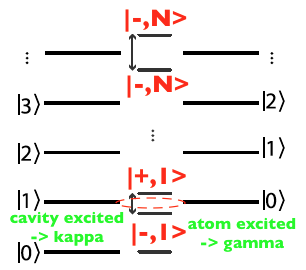
\includegraphics[height=6cm]{cavityPic2}
 	 	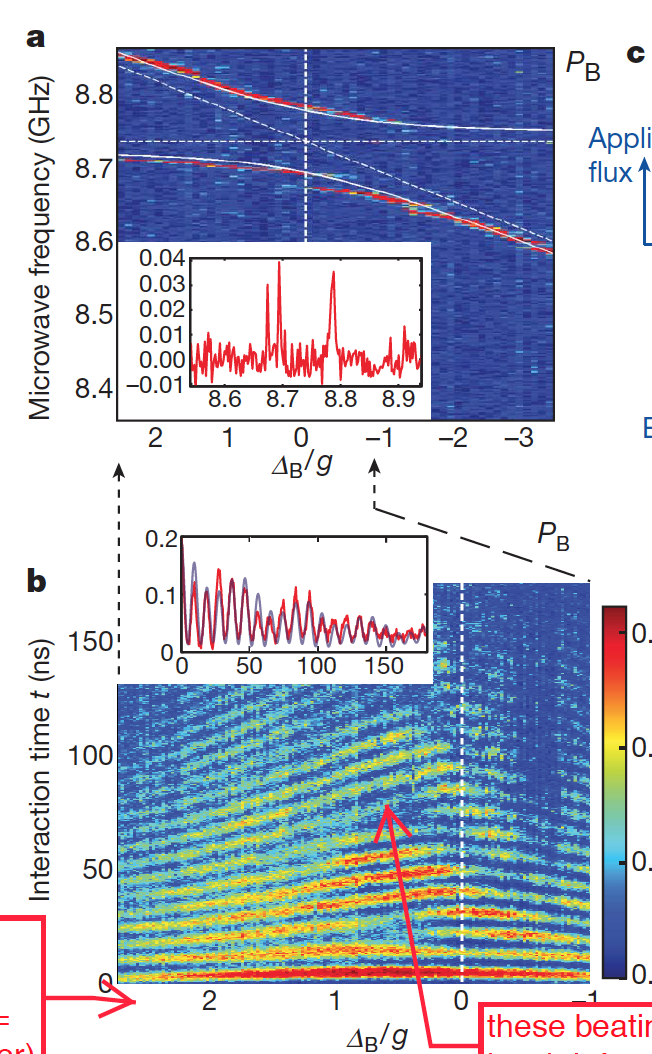
\includegraphics[height=6cm]{coherentStateStorageBetweenPhaseQubits3}
 	 	\caption{The ladder energy levels of the qubit-cavity are probed, first by direct measurement of transmission (fire in microwave and see if it hits any transitions in the system); b) Then do Rabi oscillation measuments, jumping to the first `split' level using a $ \pi $ pulse and then allowing system to evolve between the two levels. Smaller detuning $ \Delta $\ra smaller splitting between the levels \ra smaller Rabi amplitude ($ \propto \sqrt{4g^2+\Delta^2} $)\ra broader oscillations. }
 	 \end{figure}
  \newpage
  \subsection{What pulses are used?}
   \begin{itemize}
   	\item We have the microwave pulse, \textbf{that evolves the state of the qubit};
   	\item We have the DC flux shift pulse \textbf{that tunes the qubits in resonance with the cavity};
   	\item We have the RF flux shift pulse \textbf{that we use for readout};
   \end{itemize}

	\ipicCaption{8cm}{coherentStateStorageBetweenPhaseQubits4}{Detune from cavity \ra apply $ \pi- $pulse \ra interact with cavity over time $ t_A $ \ra transfer to qubit B over time $ t_B $}
	
	To understand what is happening below:
	\begin{itemize}
		\item Qubit a is prepared in state \iup\isub{A} using a $ \pi $-pulse;
		\item Qubit A is tuned in resonance with teh cavity, so that the evolution:
		\[
				U\iket{0,e} = \cos(gt_A)\iket{\iup,0} + i\sin(gt_A)\iket{\idown,1},
		\]
		\noindent takes place, transferring the excitation to the cavity state \iket{1}. \red{If we hold $ t_A $, then Rabi oscillations will occur between the cavity-qubitA states \iket{e,0} and \iket{g,1} and the probability of qubit A being excited osciilates as seen in Fig.\,a.};
		\item Qubit A is detuned, and all that we have left is some cavity state:
		\[
			\alpha\iket{0}+\beta\iket{1};
		\]
		\item Qubit B is tuned to the cavity, and a similar evolution takes place as with qubit A. Now $ t_B $ controlls the population of \iup\isub{B}. \red{So we invert Fig.a (so that we have a map of when the cavity is excited \iket{1}) and slice horizontally to recreate the Rabi oscillations between the B qubit and the cavity \ra this is seen as dots.};
	\end{itemize}
Weaker signal for longer operation times due to decay of the cavity state.
	\ipicCaption{9cm}{coherentStateStorageBetweenPhaseQubits5}{The probabilities of \iup\isub{A} and \iup\isub{B} as a function of the interaction times $ t_A $ and $ t_B $.}

 \subsection{Ramsery evolution}
  To varify that quantum coherence is maintained throughout the transfer (our phase does not drift or jump) we do Ramsay fringe experiment
  
  \ipic{6cm}{coherentStateStorageBetweenPhaseQubits6}

	\begin{itemize}
		\item Create superposed state on qubit A by driving
		
		\begin{equation}\label{app2}
		\mathcal{H} = -\frac{\hbar\omega_0}{2}\sigma_z-\hbar\Omega\cos(\omega_0 t)\sigma_x
		\end{equation}
		
		\noindent for which we shall try the unitary transformation
		
		\begin{equation}\label{app2Try}
		U(t) = \exp\left[-i\frac{\omega_0 t}{2}t\right]
		\end{equation}  
		
		\noindent resulting in the Hamiltonian 
		
		\begin{equation}\label{app2New}
		\begin{aligned}
		\mathcal{H'} & = U\mathcal{H}U^{\dagger} - i\hbar U\dot{U}^{\dagger}\\
		& = -\frac{\hbar\omega}{2}e^{-i\omega_0t/2\sigma_z}\sigma_ze^{+i\omega_0t/2\sigma_z}-\hbar\Omega\frac{e^{i\omega t}+e^{-i\omega t}}{2}e^{-i\omega_0t/2\sigma_z}\sigma_xe^{i\omega_0t/2\sigma_z}- i\hbar e^{-i\omega_0t/2\sigma_z}\bigg(i\frac{\omega}{2}\sigma_z\bigg)e^{i\omega_0t/2\sigma_z}\\
		& = -\frac{\hbar\Omega}{2}\bigg(e^{i\omega t}+e^{-i\omega t}\bigg)e^{-i\omega_0t/2\sigma_z}\red{e^{(-1)i\omega_0t/2\sigma_z}\sigma_x}\\
		& = -\frac{\hbar\Omega}{2}\bigg(e^{i\omega t}+e^{-i\omega t}\bigg){e^{-i\omega_0t\sigma_z}\sigma_x}\\
		& =-\frac{\hbar\Omega}{2}\bigg(e^{i\omega t}+e^{-i\omega t}\bigg)\begin{pmatrix}
		e^{-i\omega_0t}&0\\0&e^{+i\omega_0t}
		\end{pmatrix}\begin{pmatrix}
		0&1\\1&0
		\end{pmatrix}\\
		& =-\frac{\hbar\Omega}{2}\bigg(e^{i\omega t}+e^{-i\omega t}\bigg)\begin{pmatrix}
		0&e^{i\omega_0t}\\e^{-i\omega_0t}&0
		\end{pmatrix}
		\\
		& =-\frac{\hbar\Omega}{2}\begin{pmatrix}
		0&1+e^{2i\omega_0t}\\1+e^{-2i\omega_0t}&0
		\end{pmatrix}
		\\
		& \approx -\frac{\hbar\Omega}{2}\begin{pmatrix}
		0&1\\1&0
		\end{pmatrix}
		\\
		& \approx -\frac{\hbar\Omega}{2}\sigma_x
		\end{aligned}
		\end{equation}
		
		\noindent where we have applied the RWA where we neglect fast rotating terms (which correspond to non conserved energy processes). \iframe{Physically what we have done in entered the frame of the initial qubit Hamiltonian ($ \mathcal{H} = -\frac{\hbar\omega}{2}\sigma_z $), implicitly taking into account the raw evolution to concentrate only on the driving field contribution.}
		
		Now the evolution of the state 
		
		\begin{equation}\label{app2Ev}
		U(t) = e^{-i\mathcal{H'}/\hbar t} = e^{i\Omega t/2\sigma_x}
		\end{equation}
		
		\noindent over a time $ t = \pi/\Omega $
		
		\begin{equation}\label{app2State}
		\begin{aligned}
			\ket{\Psi_A} = U\ket{0} & = \cos(\frac{\Omega t}{2})\ket{0}+e^{i\pi/2}\sin(\frac{\Omega t}{2})\ket{1}\\
			& \red{= \frac{\iup + \idown}{\sqrt{2}}}
		\end{aligned}
		\end{equation}
		
		\item Then we couple the qubit to the cavity by applying a DC pulse, and the system will evolve according to the qubit-cavity Hamiltonian Eq.~\eqref{eqn:qubitCavityHamil} for $ N=0 $
		
		\[
			\begin{aligned}
			\mathcal{H}_\text{A-cav} & = \kbordermatrix{&\ket{\uparrow,N} & \ket{\downarrow,N+1}\\
				\bra{\uparrow,N} & \blue{\hbar\omega_A(N+\frac{1}{2}) + \hbar\Delta} & \red{\hbar g_0\sqrt{N+1}}\\
				\bra{\downarrow,N+1} & \red{\hbar g_0\sqrt{N+1}} & \blue{\hbar\omega_A(N+\frac{1}{2}) - \hbar\Delta}}\\
			& = \frac{\hbar\omega_A}{2}\mathbb{I} + \hbar g_\text{A-cav}\sigma_x + \hbar\Delta_A\sigma_z\quad\text{ignore the identity matrix, as it doesn't do anything}\\
			& \Rightarrow \quad U = e^{i\mathcal{H}t/\hbar} = e^{ig_\text{A-cav}t\sigma_x}e^{i\Delta_A t\sigma_z}\\
			& = \begin{pmatrix}
			\cos{g_\text{A-cav}t} & i\sin{g_\text{A-cav}t}\\i\sin{g_\text{A-cav}t}&\cos{g_\text{A-cav}t}
			\end{pmatrix} \begin{pmatrix}
			e^{i\Delta_A t} & 0\\0&e^{-i\Delta_A t}
			\end{pmatrix}
%			\quad\Rightarrow\quad e^{i\mathcal{H}t/\hbar}\frac{1}{\sqrt{2}}\begin{pmatrix}1 \\1 \end{pmatrix} = \frac{\iup+e^{i\phi}\idown}{\sqrt{2}}
			\end{aligned}
		\]
		
		\noindent and so the state evolves (ignoring normalisation)
		
		\[
			\begin{aligned}
			\iket{\Psi_{cav}} &= 	\begin{pmatrix}
			\cos{g_\text{A-cav}t} & i\sin{g_\text{A-cav}t}\\i\sin{g_\text{A-cav}t}&\cos{g_\text{A-cav}t}
			\end{pmatrix} \begin{pmatrix}
				e^{i\Delta_A t_A} & 0\\0&e^{-i\Delta_A t_A}
				\end{pmatrix}
				\begin{pmatrix}
							1 \\1
				\end{pmatrix}\\
				& = \begin{pmatrix}
				e^{i\Delta_A t_A} & 0\\0&e^{-i\Delta_A t_A}
				\end{pmatrix}\begin{pmatrix}
				e^{ig_\text{A-cav}t} \\e^{ig_\text{A-cav}t}\\
				\end{pmatrix} \\
				& = e^{i(g_\text{A-cav}+\Delta_A)t} \begin{pmatrix}
				1 \\e^{-2i\Delta_A t_A}\\
				\end{pmatrix} \equiv \red{\frac{\iket{e_A,0}+e^{-2i\Delta_A t_A}\iket{g_A,1}}{\sqrt{2}}}
			\end{aligned}
		\]
		
		So the state of the cavity is \[ =\frac{\iket{0}+e^{-2i\Delta_A t_A}\iket{1}}{\sqrt{2}}, \] after which we decouple the qubit
		
		\item  Next we transfer to the second qubit in exactly the same way as above (tune qubit B to the cavity and allow free evolution under the same hamiltonian as above, now with qubit B parameters
		
		\[
		\begin{aligned}
		\mathcal{H}_\text{cav-B} = & \frac{\hbar\omega_B}{2}\mathbb{I} + \hbar g_\text{cav-B}\sigma_x + \hbar\Delta_B\sigma_z\quad\text{ignore the identity matrix, as it doesn't do anything}\\
		& \Rightarrow \quad U = e^{i\mathcal{H}t/\hbar} = e^{ig_\text{cav-B}t_B\sigma_x}e^{i\Delta_B t_B\sigma_z}\\
		\end{aligned}
		\]
		
		\noindent and so the state evolves (ignoring normalisation)
		
		\[
		\begin{aligned}
		\iket{\Psi_{cav-B}} &=
		\begin{pmatrix}
		e^{i\Delta_B t_B} & 0\\0&e^{-i\Delta_B t_B}
		\end{pmatrix}\begin{pmatrix}
		e^{ig_\text{cav-B}t_B} \times 1 \\e^{ig_\text{cav-B}t_B} \times e^{-2i\Delta_At_A}
		\end{pmatrix}\\
		& = e^{i(g_\text{cav-B}+\Delta_B)t_B} \begin{pmatrix}
		1 \\e^{-2i(\Delta_A t_A+\Delta_B t_B)}\\
		\end{pmatrix} \equiv \red{\frac{\iket{e_B,0}+e^{-2i(\Delta_A t_A+\Delta_B t_B)}\iket{g_B,1}}{\sqrt{2}}},
		\end{aligned}
		\]
		
		\noindent so qubit B has a state
		
		\[
		\frac{\iket{e_B}+e^{-2i(\Delta_A t_A+\Delta_B t_B)}\iket{g_B}}{\sqrt{2}} \equiv \begin{pmatrix}
			1 \\ e^{i\Theta}
		\end{pmatrix}\quad \Theta = -2(\Delta_A t_A+\Delta_B t_B)
		\]
		
		
		\item Next we allow free evolution over time $ \Delta t $ of the decoupled second qubit:
		\[
			\begin{aligned}
			\mathcal{H_B} &= \hbar\omega_B\sigma_z \quad\Rightarrow\quad U(\Delta t) = \imatrix{e^{i\omega_B \Delta t}}{0}{0}{e^{-i\omega_B \Delta t}}\\
			\iket{\Psi_B'} & = \imatrix{e^{i\omega_B \Delta t}}{0}{0}{e^{-i\omega_B \Delta t}}\imatrixcol{1}{e^{i\Theta}} \equiv \red{\imatrixcol{1}{e^{i(\Theta - 2\omega_B \Delta t)}}}
			\end{aligned}
		\]
		
		\item Finally we apply a final $ \pi/2 $ pulse to the qubit B in a similar way to above, but with a very slight detuning:
		\[
			\begin{aligned}
						 \mathcal{H} & = \frac{\hbar\Delta\omega}{2}\sigma_z -\frac{\hbar\Omega}{2}\sigma_x\\
						U(t=\frac{\pi}{\Omega}) &= e^{i\Omega t/2\sigma_x} e^{i\Delta\omega t/2\sigma_z}= e^{i\pi/2\sigma_x} e^{i\Delta\omega \pi/2\Omega\sigma z}= i\sigma_x\imatrix{e^{i\Delta\omega \pi/2\Omega}}{0}{0}{e^{-i\Delta\omega \pi/2\Omega}}\\
						\iket{\Psi_B} & =\imatrix{e^{i\Delta\omega \pi/2\Omega}}{0}{0}{e^{-i\Delta\omega \pi/2\Omega}} i\imatrix{0}{1}{1}{0}\imatrixcol{1}{e^{i(\Theta - 2\omega_B \Delta t)}}\\
						&\equiv \imatrix{e^{i\Delta\omega \pi/2\Omega}}{0}{0}{e^{-i\Delta\omega \pi/2\Omega}} \imatrixcol{e^{i(\Theta - 2\omega_B \Delta t)}}{1},
			\end{aligned}
		\]
		
		\noindent which we see as Ramsay fringes (not the end, since you need to use the detuning between the cavity and the atom
		
		\ipic{7cm}{coherentStateStorageBetweenPhaseQubits7}
%		\[
%			\begin{aligned}
%			U\frac{\iup + \idown}{\sqrt{2}} =& \cos(gt)\mathbb{I} + i\sin(gt)\sigma_x\big]\frac{\iup + \idown}{\sqrt{2}}\\
%			& = \imatrix{\cos(gt)}{i\sin(gt)}{i\sin(gt)}{\cos(gt)}\frac{1}{\sqrt{2}}\begin{pmatrix}
%				1 \\1
%			\end{pmatrix}
%			\end{aligned}
%		\]
	\end{itemize}

\newpage
